\documentclass[12pt,a4paper]{article}
\usepackage[utf8]{inputenc}
\usepackage[margin=1in]{geometry}
\usepackage{amsmath,mathtools}
\usepackage{physics,siunitx}
\usepackage{graphicx,float}
\usepackage{tikz,empheq}
\usepackage{fancyhdr}
\usepackage{lastpage}

\pagestyle{fancy}
\lhead{Richard Whitehill}
\chead{PHYS 631 -- HW A}
\rhead{01/20/2022}
\cfoot{\thepage \hspace{1pt} of \pageref{LastPage}}

\usepackage{calligra}
\DeclareMathAlphabet{\mathcalligra}{T1}{calligra}{m}{n}
\DeclareFontShape{T1}{calligra}{m}{n}{<->s*[2.2]callig15}{}\newcommand{\scripty}[1]{\ensuremath{\mathcalligra{#1}}}
\newcommand{\script}[1]{\ensuremath{\mathcalligra{#1}}}
\newcommand{\scriptr}{\script{r}}

\newcommand{\sif}[1]{\si[per-mode=fraction]{#1}}
\newcommand{\sis}[1]{\si[per-mode=symbol]{#1}}

\newcommand{\xhat}{\hat{x}}
\newcommand{\yhat}{\hat{y}}
\newcommand{\zhat}{\hat{z}}

\newcommand{\bef}{\begin{figure}[h!]\centering}
\newcommand{\eef}{\end{figure}}

\newcommand{\eref}[1]{Eq.~(\ref{eq:#1})}
\newcommand{\erefs}[2]{Eqs.~(\ref{eq:#1})--(\ref{eq:#2})}
\newcommand{\fref}[1]{Fig.~\ref{fig:#1}}
\newcommand{\frefs}[2]{Figs.~\ref{fig:#1}--\ref{fig:#2}}
\newcommand{\tref}[1]{Table~\ref{tab:#1}}
\newcommand{\trefs}[2]{Table~(\ref{tab:#1})--(\ref{tab:#2})}

\newcommand{\prob}[2]{\textbf{#1)} #2}

\setlength{\parskip}{\baselineskip}
\setlength{\parindent}{0pt}

\begin{document}

\prob{1.5}{Prove the BAC-CAB rule by writing out both sides in component form.} 

Notice that 
\begin{align*}
\vec{B} \times \vec{C} = 
\begin{vmatrix}
\xhat & \yhat & \zhat \\
B_x & B_y & B_z \\
C_x & C_y & C_z 
\end{vmatrix}
=
\qty(B_yC_z - B_zC_y)\xhat + \qty(B_zC_x - B_xC_z)\yhat + \qty(B_xC_y - B_yC_x)\zhat,
\end{align*}
so 
\begin{align*}
\vec{A} \times \qty(\vec{B} \times \vec{C}) &= 
\begin{vmatrix}
\xhat & \yhat & \zhat \\
A_x & A_y & A_z \\
\qty(\vec{B} \times \vec{C})_x & \qty(\vec{B} \times \vec{C})_y & \qty(\vec{B} \times \vec{C})_z 
\end{vmatrix} 
\end{align*}
\begin{empheq}[box=\fbox]{align*}
\vec{A} \times \qty(\vec{B} \times \vec{C}) = &\qty[A_y\qty(B_xC_y - B_yC_x) - A_z\qty(B_zC_x - B_xC_z)]\xhat \\
+ &\qty[A_z\qty(B_yC_z - B_zC_y) - A_x\qty(B_xC_y - B_yC_z)]\yhat \\
+ &\qty[A_x\qty(B_zC_x - B_xC_z) - A_y\qty(B_yC_z - B_zC_y)]\zhat
\end{empheq}

Next, note that
\begin{align*}
\vec{B}\qty(\vec{A} \cdot \vec{C}) - \vec{C}\qty(\vec{A} \cdot \vec{B}) &= \qty(A_xC_x + A_yC_y + A_zC_z)\qty(B_x\xhat + B_y\yhat + B_z\zhat) \\
&- \qty(A_xB_x + A_yB_y + A_zB_z)\qty(C_x\xhat + C_y\yhat + C_z\zhat)
\end{align*}
\begin{empheq}[box=\fbox]{align*}
\vec{B}\qty(\vec{A} \cdot \vec{C}) - \vec{C}\qty(\vec{A} \cdot \vec{B}) &= \qty[B_xA_yC_y + B_xA_zC_z - C_xA_yB_y - C_xA_zB_z]\xhat \\
&+ \qty[B_yA_xC_x + B_yA_zC_z - C_yA_xB_x - C_yA_zB_z]\yhat \\
&+ \qty[B_zA_xC_x + B_zA_yC_y - C_zA_xB_x - C_zA_yB_y]\zhat.
\end{empheq}
It can be easily observed that $\vec{A} \times \qty(\vec{B} \times \vec{C}) = \vec{B}\qty(\vec{A} \cdot \vec{C}) - \vec{C}\qty(\vec{A} \cdot \vec{B})$ by comparing terms component-wise.

Alternatively,
\begin{align*}
\qty(\vec{A} \times \qty(\vec{B} \times \vec{C}))_{i} &= \epsilon_{ijk}A_j\qty(\vec{B} \times \vec{C})_{k} = \epsilon_{ijk}\epsilon_{klm}A_jB_lC_m \\
&= \qty(\delta_{il}\delta_{jm} - \delta_{im}\delta_{jl})A_jB_lC_m \\
&= B_i\qty(A_jC_j) - C_i\qty(A_iB_i) \\
\Rightarrow \vec{A} \times \qty(\vec{B} \times \vec{C}) &= \vec{B}\qty(\vec{A} \cdot \vec{C}) - \vec{C}\qty(\vec{A} \cdot \vec{B}).
\end{align*}


\prob{1.6}{Prove that $\qty[\vec{A} \times \qty(\vec{B} \times \vec{C})] + \qty[\vec{B} \times \qty(\vec{C} \times \vec{A})] + \qty[\vec{C} \times \qty(\vec{A} \times \vec{B})] = 0$. Under what conditions does $\vec{A} \times \qty(\vec{B} \times \vec{C}) = \qty(\vec{A} \times \vec{B}) \times \vec{C}$?}

From the BAC-CAB rule, we have
\begin{empheq}[box=\fbox]{align*}
\qty[\vec{A} \times \qty(\vec{B} \times \vec{C})] + \qty[\vec{B} \times \qty(\vec{C} \times \vec{A})] + \qty[\vec{C} \times \qty(\vec{A} \times \vec{B})] &= \vec{B}\qty(\vec{A} \cdot \vec{C}) - \vec{C}\qty(\vec{A} \cdot \vec{B}) \\
&+ \vec{C}\qty(\vec{B} \cdot \vec{A}) - \vec{A}\qty(\vec{B} \cdot \vec{C}) \\
&+ \vec{A}\qty(\vec{C} \cdot \vec{B}) - \vec{B}\qty(\vec{C} \cdot \vec{A}) \\
&= 0,
\end{empheq}
since the dot product is commutative.

Notice that $\vec{A} \times \qty(\vec{B} \times \vec{C}) = \qty(\vec{A} \times \vec{B}) \times \vec{C}$ whenever $\vec{B} \times \qty(\vec{C} \times \vec{A})$ is zero.
Thus, $\vec{B} \cdot \qty(\vec{C} \times \vec{A}) = $, meaning that $\vec{B}$ and $\vec{C} \times \vec{A}$ are scalar multiples of each other.
Geometrically, $\vec{B}$ is normal to the plane spanned by $\vec{A}$ and $\vec{C}$.

\bef
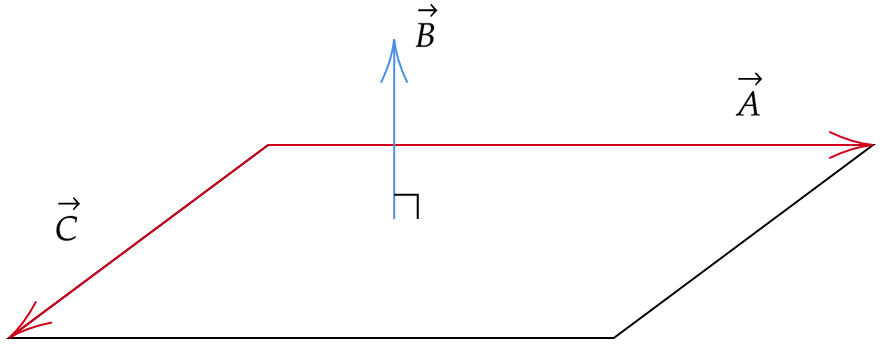
\includegraphics[scale=0.3]{./fig1.png}
\eef

\end{document}
